\apendice{Plan de Proyecto Software}

\section{Introducción}

En este documento se pretende mostrar el plan de proyecto seguido a la hora de realizar el trabajo de fin de grado.

Debido al auge de las metodologías ágiles en la industria y sus indiscutibles ventajas, se ha escogido la metodología Scrum para desarrollar el proyecto. Los conceptos teóricos seguidos se encuentran en el <<Manual de Scrum>>~\cite{scrumMaster2022}, temario necesario para obtener la certificación de Scrum Manager.

Posteriormente, se expondrá la viabilidad legal y económica del producto.

\section{Scrum}

Scrum es una metodología ágil basada en cuatro valores~\cite{scrumMaster2022}. Sintetizando sus principios, se puede deducir que se pretende valorar a los individuos por encima de las herramientas, el \textit{software} apropiado a la documentación exhaustiva, la colaboración con el cliente y la habilidad de dar respuesta al cambio ante imprevistos.

Siguiendo este esquema, se desarrolla el <<ciclo de Scrum>> representado en la imagen~\ref{img:ciclo_scrum}, que se puede dividir en varios pilares.

\begin{figure}[h]
	\caption[Resumen del ciclo de Scrum]{Resumen del ciclo de Scrum según el Manual de Scrum~\cite{scrumMaster2022}.}
	\label{img:ciclo_scrum}
	\centering
	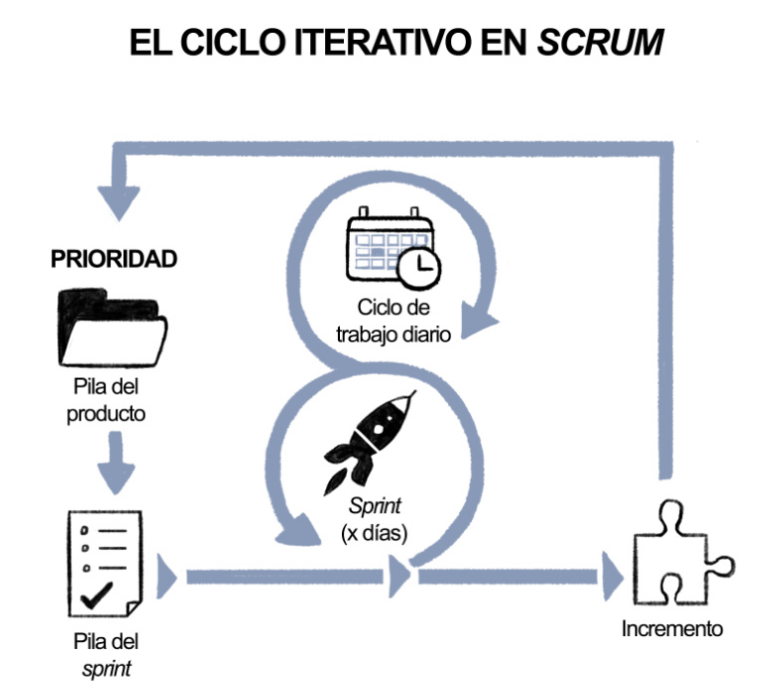
\includegraphics[scale=0.45]{../img/anexos/scrum/ciclo}
\end{figure}

\subsection{Roles}
Descripción de los posibles interventores durante el desarrollo de un producto.

\begin{itemize}
	\item \textit{Product owner}: es el representante del cliente, y su responsabilidad es el valor del producto. Es quien gestiona la pila del producto (conjunto de historias de usuario solicitadas por el cliente), así como la prioridad de cada ítem que lo compone.
	
	\item Scrum \textit{master}: es el responsable de garantizar que el proyecto se desarrolla siguiendo los principios de Scrum, asesorando a los desarrolladores. También es el moderador en las reuniones diarias de Scrum y el encargado de resolver dinámicas que puedan perjudicar al equipo.
	
	\item Equipo de desarrollo: es el conjunto de programadores autogestionados encargados de generar los incrementos. Profesionales multifuncionales, deben completar las tareas que se les asignen en el plazo estimado, además de participar en la toma de decisiones.
\end{itemize}

\subsection{Artefactos}

Son las <<herramientas>>~\cite{scrumMaster2022} elementales. Entre ellos se encuentran:

\begin{itemize}
	\item Pila de producto o \textit{product backlog}: contiene las historias de usuario (el equivalente a los <<requisitos>> en las metodologías tradicionales). Evoluciona durante el proyecto en función de las peticiones del cliente.
	\item Pila del \textit{sprint} o \textit{sprint backlog}: es la lista de tareas que han de completar los desarrolladores en un \textit{sprint}. En este proyecto, se han utilizado las \textit{milestones} de GitHub (asignándoles \textit{issues}) para representarla.
	\item Incremento: resultado de cada \textit{sprint}. Ha de ser un entregable.
	\item Gráfico de avance o \textit{burn down report}: muestra el trabajo pendiente por realizar en un \textit{sprint} y es actualizado por los desarrolladores. Indica, además, el ritmo de trabajo <<ideal>> que se debería seguir para alcanzar los objetivos. En este caso, se ha utilizado el gráfico generado por ZenHub.
	\item Gráfico de producto o \textit{burn up report}: mide cuánto se ha completado respecto al total.
\end{itemize}

\subsection{Eventos}
Durante el ciclo de Scrum, se pueden identificar varias actividades que constituyen la rutina y se represetan en la imagen~\ref{img:eventos_scrum} facilitada por el Manual de Scrum~\cite{scrumMaster2022}.

\begin{figure}[h]
	\caption[Eventos de Scrum]{Eventos de Scrum según el Manual de Scrum~\cite{scrumMaster2022}.}
	\label{img:eventos_scrum}
	\centering
	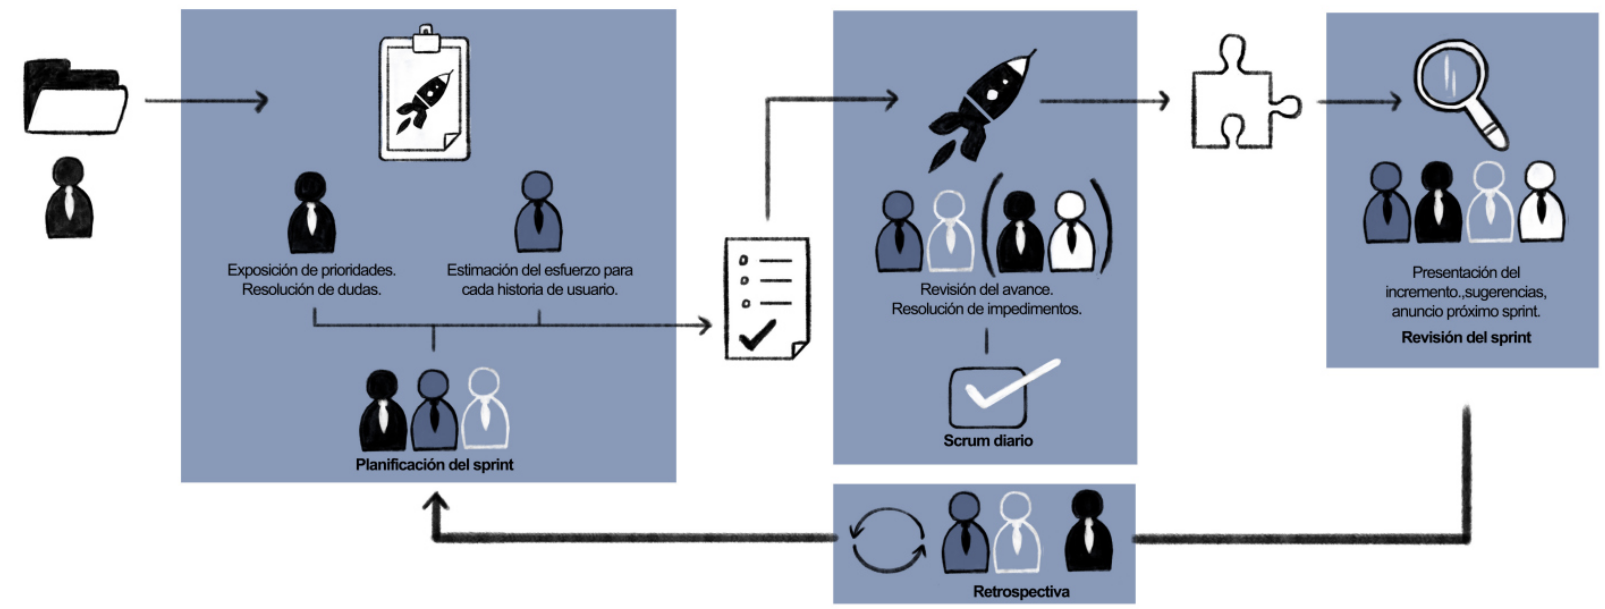
\includegraphics[width=\textwidth]{../img/anexos/scrum/eventos}
\end{figure}

\begin{enumerate}
	\item \textit{Sprint} o iteración: es un periodo de tiempo fijo (y breve) en el que se trabaja para completar una cantidad de tareas prefijadas con antelación (la pila del \textit{sprint}). Se han utilizado los \textit{sprints} de ZenHub para realizar el seguimiento.
	\item Reunión de planificación sel \textit{sprint}: marca el inicio de cada \textit{sprint} y determina las tareas a desarrollar, además de su duración temporal.
	\item Scrum diario: breve reunión en la que cada integrante del equipo notifica su ritmo de trabajo con el fin de corregir posibles impedimentos que ralenticen el ciclo. Además, se actualiza el \textit{burndown report}. En este caso, debido a que el equipo está formado únicamente por un desarrollador, se ha omitido.
	\item Revisión del \textit{sprint}: se analiza el incremento entregado y se adapta la pila del producto en caso de necesitarlo (por ejemplo, si se ha encontrado algún \textit{bug} o se necesita refactorizar).
	\item Retrospectiva del \textit{sprint}: se aporta el \textit{feedback} necesario para mejorar la siguiente iteración.
\end{enumerate}

\subsection{Medición}

Como se puede observar, cada equipo puede realizar una cantidad de trabajo, generalmente fija, en cada \textit{sprint}. Por ello, es necesario estimar el tiempo que requiere cada tarea y no asignar más trabajo del que se pueda asimilar en cada iteración.

En este proyecto, se han utilizado los <<puntos de historia>> como unidad de medida.


\section{Planificación temporal}

\subsection{Planificación por \textit{sprints}}
\label{s:planificacion-sprints}
Siguiendo los eventos de Scrum, y adaptándolos teniendo en cuenta el tamaño del equipo (un desarrollador), se ha decidido planificar el proyecto mediante \textit{sprints}.

\subsubsection{\textit{Sprint 1: Mustard}}

\begin{itemize}
	\item \textbf{\textit{Planning meeting}}
	
	Durante la reunión se marcaron los siguientes objetivos:
	
	\begin{enumerate}
		\item Configuración básica: incluyendo la creación del repositorio, la correcta instalación de ZenHub, la creación de entornos virtuales (miniconda, Scikit-Learn, etc.) y la familiarización con conceptos Scrum: \textit{milestones, sprints, epics}, etc.
		\item Memoria: comienzo de la redacción incluyendo las secciones de introducción, conceptos teóricos (aprendizaje automático) y trabajo relacionado.
		\item Investigación: búsqueda del código SSADR-CoF y de las bases de datos utilizadas en el paper.
		\item Lectura de papers: Engelen \& Hoos~\cite{engelen2020surveyOnSemiSupervised}, García, Triguero \& Herrera~\cite{triguero2015SelflabeledTechniques}, y Zhou \& Duan~\cite{zhou2021SemisupervisedRecommendationAttack}.
	\end{enumerate}
	
	\item \textbf{Marcas temporales}
	
	El \textit{sprint} se desarrolló entre el 24 de septiembre de 2022 y el 2 de octubre del 2022.
	
	\item \textbf{\textit{Burndown Report}}
	\begin{figure}[h]
		\caption{\textit{Burndown Report Sprint 01}}
		\centering
		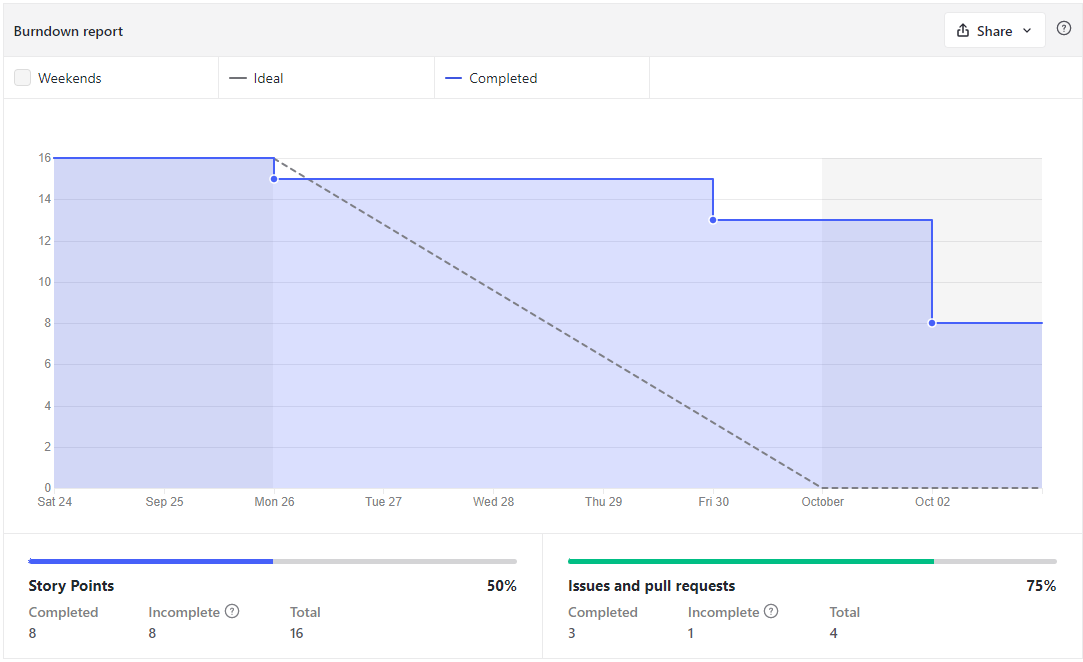
\includegraphics[width=\textwidth]{../img/anexos/bdr/s01_bdr}
	\end{figure}
	
	Como se puede comprobar, no todos los objetivos marcados fueron cumplidos: la estimación del tiempo fue demasiado optimista, además de no contar con el tiempo requerido en solucionar problemas técnicos (\LaTeX{}). Se dejó para próximos sprints la lectura del último paper.

	\item \textbf{\textit{Sprint review meeting}}
	
	Durante la reunión se fijaron ciertas correcciones en la memoria (mejorar referencias bibliográficas y la sección de <<Trabajos relacionados>>), además de la necesidad de introducir una sección teórica de ataques a los sistemas de recomendación.
	
\end{itemize}


\subsubsection{\textit{Sprint 2: Paprika}}
\begin{itemize}
	\item \textbf{\textit{Planning meeting}}
	Objetivos del siguiente Sprint:
	
	\begin{enumerate}
		\item Configuración: debido a la gran cantidad de tiempo invertida en solucionar errores de compilación en \LaTeX{}, se decidió migrar el proyecto a una nueva instalación basada en Debian.
		\item Correcciones: aspectos estilísticos y completar información.
		\item Lectura: Mingdan y Qingshan~\cite{mingdan2018ShillingAttacksAReview} con el objetivo de introducir una sección teórica de ataques.
		\item Memoria: redacción completa de los modelos de ataque en los aspectos teóricos.
		
	\end{enumerate}
	
	\item \textbf{Marcas temporales}
	
	El \textit{sprint} se desarrolló entre el 3 de octubre de 2022 y el 18 de octubre del 2022.
	
	\item \textbf{\textit{Burndown Report}}
	\begin{figure}[h]
		\caption{\textit{Burndown Report Sprint 02}}
		\centering
		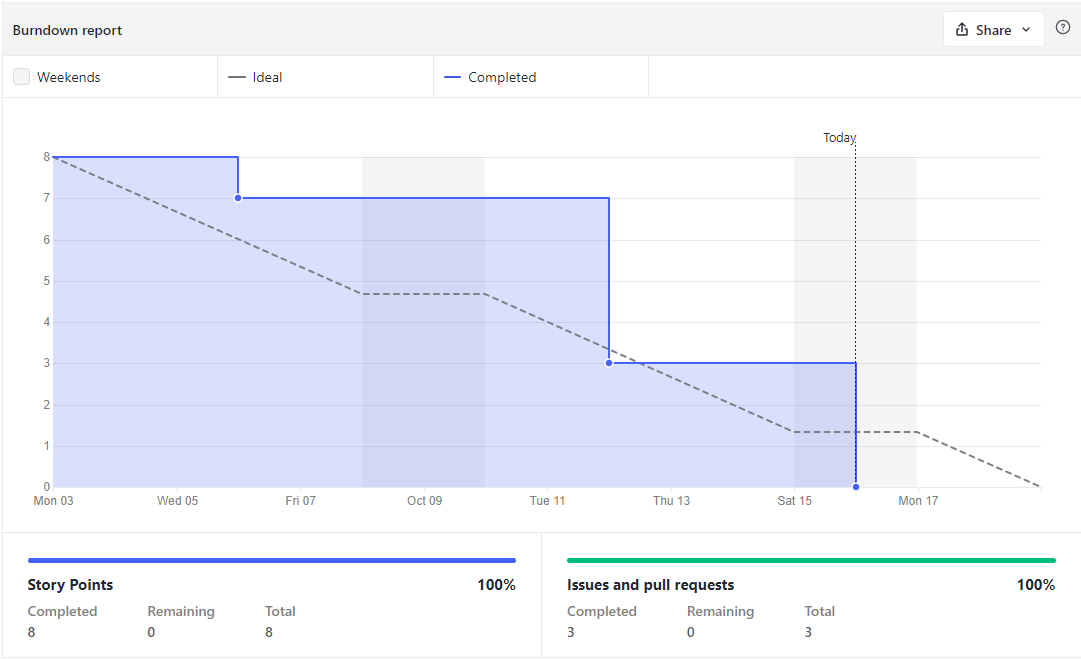
\includegraphics[width=\textwidth]{../img/anexos/bdr/s02_bdr}
	\end{figure}
		
	En este \textit{sprint} sí se cumplió con los objetivos marcados. Sin embargo, la estimación de tiempo tampoco fue la adecuada, requiriendo más de lo previsto.
	
	\item \textbf{\textit{Sprint review meeting}}
	
	Durante la reunión se resolvieron dudas acerca de bibliografía, referencias y trabajo previo. Además, se acordó empezar a programar, definiendo así los \textit{issues} desarrollados en el siguiente \textit{sprint}.
	
\end{itemize}

\subsubsection{\textit{Sprint 3: Fennel Seeds}}
\begin{itemize}
	\item \textbf{\textit{Planning meeting}}
	
	Durante esta reunión, se decidió empezar a programar el \textit{co-forest}. Para ello, se definieron los siguientes pasos:
	
	\begin{enumerate}
		
		\item Librerías: se acordó aprender a utilizar las librerías más comunes en el \textit{data science}. Entre ellas: MatplotLib y Scikit-Learn. Además, se requirió la correcta configuración del entorno virtual, haciendo que el tiempo dedicado al \textit{issue} fuese mayor de lo estimado (problemas en el \texttt{PATH} y con las dependencias).
		
		\item \textit{SKLearn}: aprovechando la correcta documentación de la librería, se decidió repasar los conceptos teóricos básicos, además del manejo de la <<interfaz>> (métodos comunes). Entre ellos:
		
		\begin{itemize}
			\item \textit{Decision trees}
			\item \textit{Self training}
			\item \textit{Random Forest}
		\end{itemize}
	
		\item Lectura: se concertó la relectura del artículo de Zhou~\cite{zhou2021SemisupervisedRecommendationAttack} con la intención de comprender el algoritmo y del \textit{paper} <<original>> del \textit{co-forest}~\cite{originalCoForest2007}. Durante el proceso de programación, además, se encontró la tesis de Van Engelen~\cite{engelen2018thesis} y se añadió al conjunto.
		\item Documentación: se acordó la corrección de los errores previamente señalados y la inclusión del \textit{sprint} en los anexos.
		\item Programación del \textit{co-forest}: se programó el pseudocódigo ilustrado en la Tesis de Van Engelen~\cite{engelen2018thesis}, que es muy similar al original~\cite{originalCoForest2007} pero con algunas diferencias. Inicialmente se intentó usar el \textit{random forest} de Scikit-Learn, pero se descartó la idea debido a la poca versatilidad que se ofrecía para manejar los \textit{concomitant ensembles}. Se han de corregir ciertos factores, pero se pospondrá hasta la correcta discusión con el tutor.
		
	\end{enumerate}
	
	\item \textbf{Marcas temporales}	
	
	El \textit{sprint} se desarrolló entre el 19 de octubre de 2022 y el 2 de noviembre del 2022.
	
	\item \textbf{\textit{Burndown Report}}
	
		\begin{figure}[h]
		\caption{\textit{Burndown Report Sprint 03}}
		\centering
		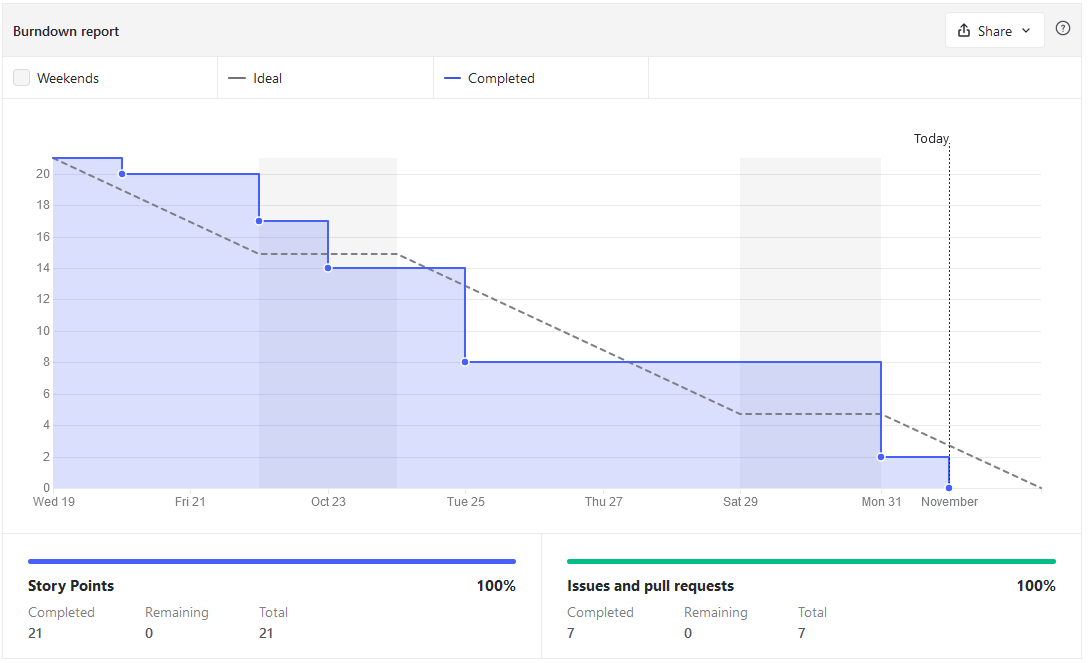
\includegraphics[width=\textwidth]{../img/anexos/bdr/s03_bdr}
		\end{figure}
	
	En este \textit{sprint} se cumplió con los objetivos marcados. Nuevamente, la estimación del tiempo fue inferior a la real (se pensaba que se podría depender más de librerías existentes de lo que se pudo en realidad), calculándose un total de aproximadamente 25 horas reales.

	\item \textbf{\textit{Sprint review meeting}}
	
	Durante la revisión del \textit{sprint}, se llegó a la conclusión de que el pseudocódigo podía ser mejor implementado aprovechando ciertas librerías de Python. Se comentó cómo mejorar complejidades espaciales y reducir el código. Se fijaron objetivos para las próximas semanas.
	
\end{itemize}


\subsubsection{\textit{Sprint 4: Cayenne}}
\begin{itemize}
	\item \textbf{\textit{Planning meeting}}
	
	Durante la reunión se acordaron los siguientes objetivos:
	
	\begin{enumerate}
		\item Reimplementación del código: se acordó volver a programar el \textit{co-forest}, esta vez implementando una versión más <<\textit{pythonizada}>> con el fin de mejorar la complejidad espacial y facilitar la lectura.
		\item Curso de Numpy: se decidió que sería interesante la realización de un curso para aprender a utilizar la librería y aplicarla al código.
		\item Curso de Pandas: aprovechando la relación con el punto anterior, se acordó completar también un curso de esta librería.
		\item Memoria: corregir aspectos anteriores e incluir toda la teoría relacionada con el \textit{co-forest}.
	\end{enumerate}
	
	\item \textbf{Marcas temporales}
	
	El \textit{sprint} se desarrolló entre el 3 de noviembre de 2022 y el 15 de noviembre del 2022.
			
	\item \textbf{\textit{Burndown Report}}
	\begin{figure}[h]
		\caption{\textit{Burndown Report Sprint 04}}
		\centering
		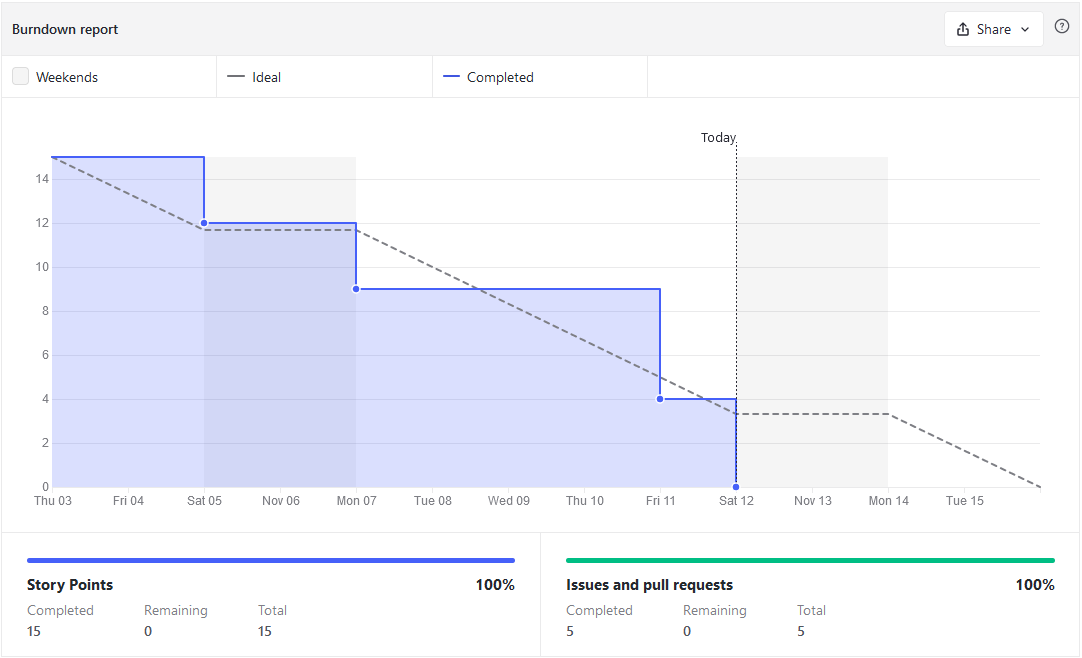
\includegraphics[width=\textwidth]{../img/anexos/bdr/s04_bdr}
	\end{figure}
	
	En este \textit{sprint} se completaron los objetivos, aunque quedaron pendientes ciertos aspectos a comentar respecto al código. Destacar que, debido a que se terminaron antes de lo planeado los \textit{issues} planificados, se aprovechó para modificar ciertos aspectos pendientes relacionados con la memoria y para probar correctamente el código. Esto hizo que el tiempo real dedicado haya sido ligeramente superior al estimado (más tiempo de documentación).
	
	\item \textbf{\textit{Sprint review meeting}}
	
	En la reunión se acordó experimentar con el algoritmo utilizando distintos conjuntos de datos, además de mejorar ciertos detalles de implementación.
	
\end{itemize}

\subsubsection{\textit{Sprint 5: Curry}}

\begin{itemize}
	\item \textbf{\textit{Planning meeting}}
	
	Durante la reunión se acordaron los siguientes objetivos:
	
	\begin{enumerate}
		\item Ajustes al código: se acordó mejorar algunos factores, como la generación de objetos <<aleatorios>> para obtener resultados deterministas en los experimentos, optimización de memoria o corrección de parámetros.
		\item Experimentación: se determinó probar el código con distintos conjuntos de datos en diferentes fases: durante el entrenamiento y tras terminarlo. Para ello, se estudiaron algunos conceptos teóricos y el uso de la librería MatplotLib para representar gráficamente los resultados obtenidos.
		\item Memoria: documentación de los experimentos realizados y correcciones.
	\end{enumerate}

	\item \textbf{Marcas temporales}		
	
	El \textit{sprint} se desarrolló entre el 15 de noviembre de 2022 y el 25 de noviembre del 2022.
	
	\item \textbf{\textit{Burndown Report}}
		\begin{figure}[h]
		\caption{\textit{Burndown Report Sprint 05}}
		\centering
		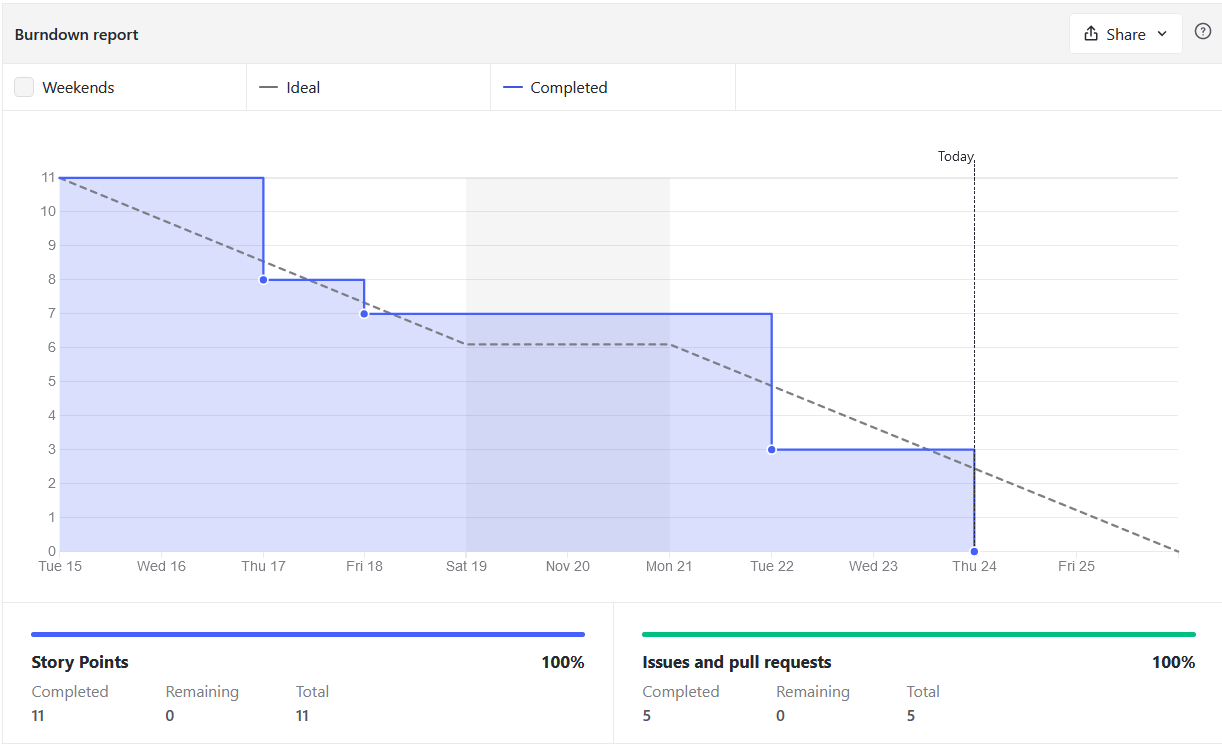
\includegraphics[width=\textwidth]{../img/anexos/bdr/s05_bdr}
	\end{figure}
	
	En este \textit{sprint} se cerraron todos los puntos de historia propuestos. Aunque se estimaron 11 horas de trabajo, el tiempo invertido fue superior, realizando 15. La mayor dedicación se justifica por la existencia de reuniones intermedias y de <<defectos>> encontrados en el código en el trascurso del \textit{sprint}.
	
	\item \textbf{\textit{Sprint review meeting}}

	Durante la reunión se acordó comparar los resultados obtenidos con los de otras herramientas, además de empezar el tratamiento de los conjuntos de datos utilizados en el \textit{paper}~\cite{zhou2021SemisupervisedRecommendationAttack}.
	
\end{itemize}


\subsubsection{\textit{Sprint 6: Coriander}}
\begin{itemize}
	\item \textbf{\textit{Planning meeting}}
	
	Durante la reunión se fijaron los siguientes objetivos:
	
		\begin{enumerate}
		\item Ajustes en las gráficas: arreglar detalles menores en el formato de ciertos gráficos.
		\item Comparativas: probar los resultados obtenidos y compararlos la herramienta de la Universidad de Granada llamada KEEL.
		\item \textit{Datasets} <<reales>>: probar el algoritmo utilizando MovieLens, una de las bases de datos utilizadas en el \textit{paper}~\cite{zhou2021SemisupervisedRecommendationAttack}. Para ello, es necesaria una re-lectura del artículo y realizar el procesamiento inicial de los datos.
		\item Memoria: documentación de los experimentos realizados.
	\end{enumerate}

	\item \textbf{Marcas temporales}	
		
	El \textit{sprint} se desarrolló entre el 25 de noviembre de 2022 y el 5 de diciembre del 2022.
	
	\item \textbf{\textit{Burndown Report}}
		\begin{figure}[h]
			\caption{\textit{Burndown Report Sprint 06}}
			\centering
			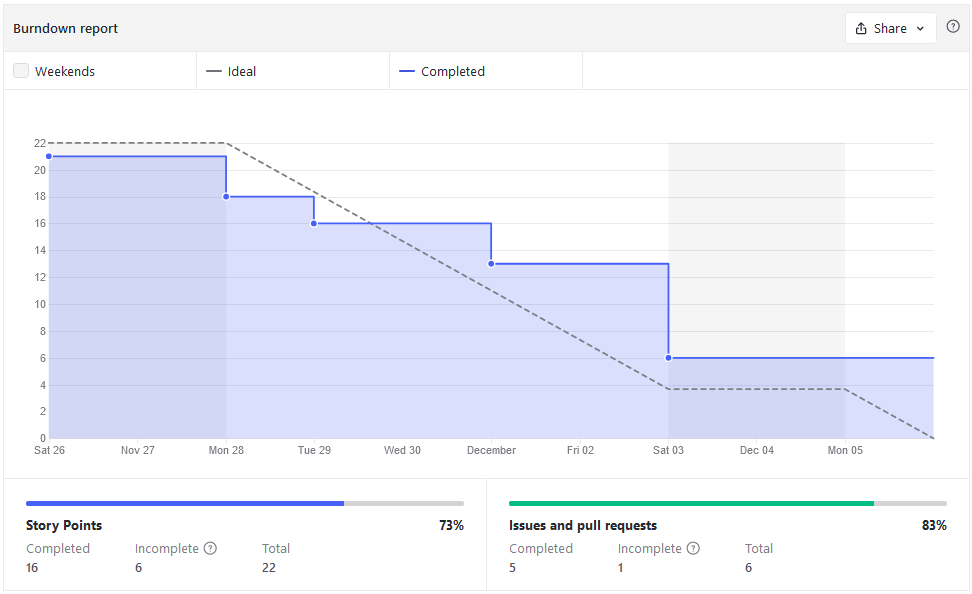
\includegraphics[width=\textwidth]{../img/anexos/bdr/s06_bdr}
		\end{figure}
	
	Puede parecer que los puntos de historia fueron mal estimados debido a que el ritmo de trabajo es bajo. Sin embargo, se justifica debido a que durante la experimentación (en concreto, durante la comparativa contra KEEL) se encontraron dos \textit{bugs} en el código (causados no por la lógica del programa, sino por el operador \textit{in} de Python y por no estar preparado para recibir etiquetas que no comiencen en 0).
	
	Debido a que los errores se encontraron una vez se realizó toda la documentación, se tuvo que repetir la sección asociada a los experimentos del \textit{co-forest}, además de localizar y depurar los errores de código. Todo este trabajo supuso un esfuerzo extra de 7 horas, que fueron introducidas en el \textit{backlog} del \textit{sprint} a mediados del mismo (debido a la gran importancia que tienen y la influencia en pasos posteriores). Por este motivo, no se completaron los objetivos previstos. Sin embargo, el tiempo dedicado al proyecto fue el estimado.
	
	Es destacable también que de los 6 puntos de historia que quedan se realizaron 2, pero se decidió dejar el \textit{issue} abierto para el siguiente \textit{sprint}.

	\item \textbf{\textit{Sprint review meeting}}
	
	Habiendo finalizado el modelo, se decidió empezar a experimentar con bases de datos de sistemas de recomendación. Además, se acordó añadir nuevas gráficas.
\end{itemize}

\subsubsection{\textit{Sprint 7: Cinnamon }}
\begin{itemize}
	\item \textbf{\textit{Planning meeting}}
	
	Se marcaron los siguientes objetivos para el \textit{sprint}.
	
	\begin{enumerate}
		\item Extraer vectores de características: estudiar e implementar el método de extracción de vectores por ventanas expuesto en el \textit{paper} de Zhou y Duan~\cite{zhou2021SemisupervisedRecommendationAttack}. Generar ficheros \texttt{.csv} con dichos vectores para poder importarlos posteriormente con Pandas. Probar la correcta generación de vectores con perfiles verdaderos y atacantes.
		\item Generación de reseñas de atacantes: siguiendo los modelos estadísticos, generar reseñas de ataque para el \textit{random attack}, el \textit{average attack} y el \textit{bandwagon attack}.
		\item Documentación: añadir introducción y descripción de Scrum en los anexos. Corregir las sugerencias anteriores. Incluir la descripción del método de extracción de vectores de características por ventanas y la generación de reseñas de atacantes.
	\end{enumerate}
	
	\item \textbf{Marcas temporales}		
	
	El \textit{sprint} se planificó para desarrollarse entre el 8 y el 20 de diciembre de 2022. Sin embargo y debido al ritmo de trabajo, se cerró el 15 de diciembre de 2022.
	
	\item \textbf{\textit{Burndown Report}}
	\begin{figure}[h]
		\caption{\textit{Burndown Report Sprint 07}}
		\centering
		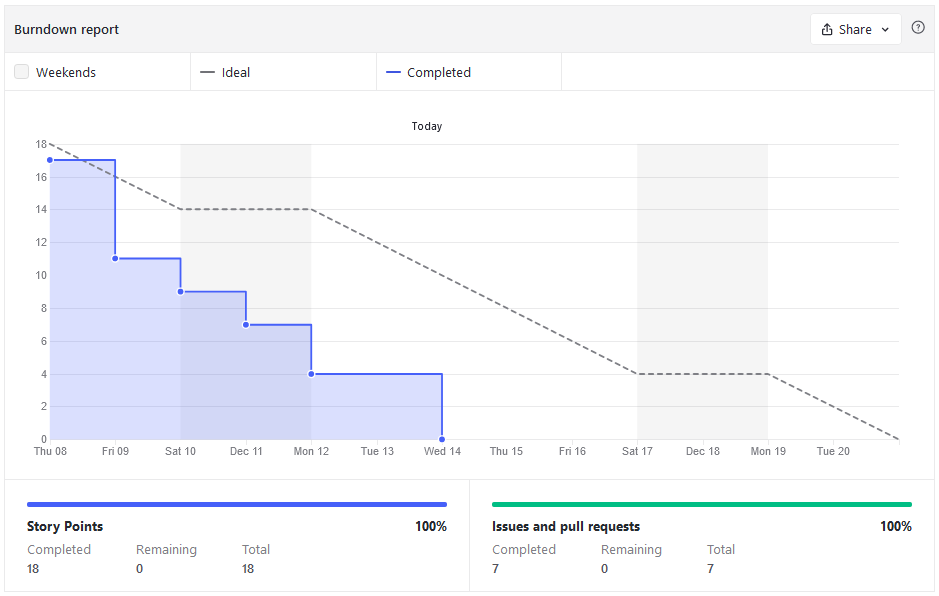
\includegraphics[width=\textwidth]{../img/anexos/bdr/s07_bdr}
	\end{figure}

	Como se puede comprobar, se finalizaron las tareas del \textit{sprint} antes de lo previsto. En gran parte, debido a que el \textit{issue} de extracción de vectores de características estaba ya comenzado en el \textit{sprint} anterior, y requirió menos tiempo del planificado. Además, el resto de tareas no dieron problemas en esta iteración. Debido a que Scrum no permite añadir nuevos ítems en la pila del \textit{sprint} durante el desarrollo de este, se decidió cerrar y comenzar uno nuevo.

	\item \textbf{\textit{Sprint review meeting}}
	
	Durante la reunión se concluyó que la forma de generar vectores de características y reseñas de ataques es correcta, por lo que se decidió experimentar con el \textit{co-forest} y datos reales.
	
\end{itemize}



\subsubsection{\textit{Sprint 8: Kaffir Lime Leaves}}
\begin{itemize}
	\item \textbf{\textit{Planning meeting}}
	
	Durante este \textit{sprint} se fijaron los siguientes objetivos:
			\begin{enumerate}
			\item Refactorizar el extractor de vectores de características y el generador de reseñas de atacantes: debido a que la sintetización de los conjuntos de entrenamiento y \textit{test} requiere demasiado tiempo ($25h$), se ha decidido mejorar la complejidad algorítmica y convertir a clase con el fin de reducir llamadas con mayor complejidad temporal. Se redujo el tiempo requerido a ($10h$) mediante el uso de la nueva estructura (en lugar de fichero de utilidades).
			\item Completar el \textit{co-forest}: añadir nuevos métodos para realizar comparaciones (predicción con probabilidades, AUC, \textit{recall} y precisión).
			\item Orden de repositorio: lectura acerca de la creación de módulos en python, conversión de los \textit{notebooks} a archivos \texttt{.py} importables, configuración de rutas.
			\item Análisis de resultados: analizar los resultados en busca de posibles errores cometidos durante la experimentación.
			\item Generación de gráficas y comparación contra \textit{random forest}: utilizando clases de Scikit-Learn, automatizar la generación de gráficas para imitar el experimento realizado por Zhou y Duan~\cite{zhou2021SemisupervisedRecommendationAttack} para el \textit{co-forest} y dos \textit{random forest} con distintos conjuntos de entrenamiento.
			\end{enumerate}
		
	\item \textbf{Marcas temporales}	
	
	Para evitar solapamientos con el \textit{sprint} anterior, oficialmente (en el repositorio) se desarrolló entre el 18 y el 22 de diciembre del 2022. Sin embargo, se empezó unos días antes.	
	
	\item \textbf{\textit{Burndown Report}}
	
	\begin{figure}[h]
		\caption{\textit{Burndown Report Sprint 08}}
		\centering
		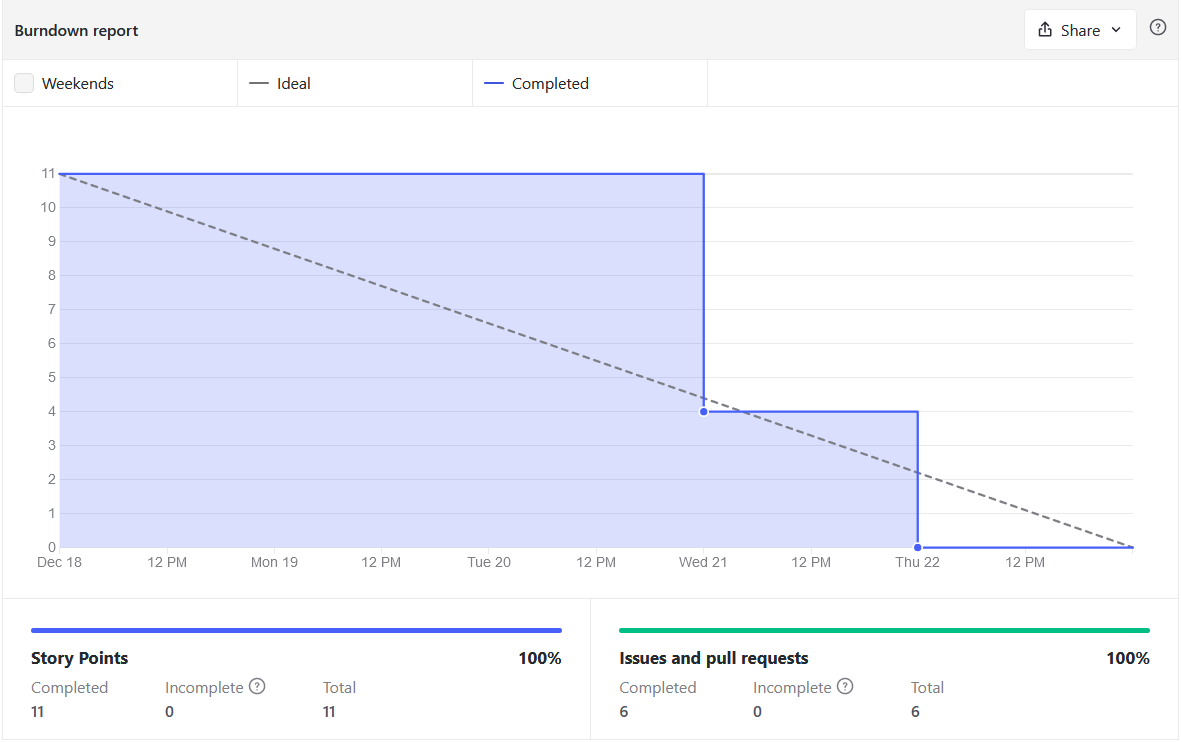
\includegraphics[width=\textwidth]{../img/anexos/bdr/s08_bdr}
	\end{figure}

	Como se puede comprobar, los \textit{issues} fueron completados correctamente.	

	\item \textbf{\textit{Sprint review meeting}}
	
	Durante la reunión se comprobó que los resultados obtenidos en la fase de experimentación no se asemejan a los presentados en el \textit{paper} seguido~\cite{zhou2021SemisupervisedRecommendationAttack}. Sin embargo, se concluyó que podrían ser correctos. Para evitar realizar afirmaciones erróneas, se decidió revisar todo el proceso de experimentación.
\end{itemize}



\subsubsection{\textit{Sprint 9: Ginger}}
\begin{itemize}
	\item \textbf{\textit{Planning meeting}}
	
	Debido a que este \textit{sprint} se realizó durante la época vacacional, se decidió realizar una revisión general del documento completando aspectos pendientes.
	
	\begin{enumerate}
		\item Experimentación \textit{co-forest}: se incluyó una gráfica \textit{extra} pendiente (tiempo de entrenamiento-número de árboles) y se repitió la experimentación esta vez utilizando conjuntos estratificados. Se corrigieron los cambios surgidos y actualizaron las gráficas en la memoria. Se revisó la clase del \textit{co-forest} y se terminó de documentar, además de adaptar los métodos a la interfaz de SKLearn (cambio de firma).
		\item Documentación: se decidió cerrar aspectos pendientes. Entre ellos: completar las secciones teóricas de semisupervisado, ensembles y métricas, repetir gráficas e ilustraciones incorrectas, revisar la bibliografía y trabajos relacionados, completar los anexos y corregir aspectos menores.
		\item Revisión de la detección de ataques: debido a que los resultados obtenidos no son los esperados, se decidió revisar toda la generación de reseñas de atacantes, extracción de perfiles y métodos de experimentación en busca de posibles errores. Se incluyeron alternativas para la AUC (curva \textit{precision} - \textit{recall}).
		\item Implementación: se investigó acerca del \textit{tri-training} y se implementó este nuevo método.
	\end{enumerate}

	\item \textbf{Marcas temporales}		
	
	El \textit{sprint} se desarrolló entre el 27 de diciembre del 2022 y el 8 de enero del 2023.
	
	\item \textbf{\textit{Burndown Report}}
	\begin{figure}[h]
		\caption{\textit{Burndown Report Sprint 09}}
		\centering
		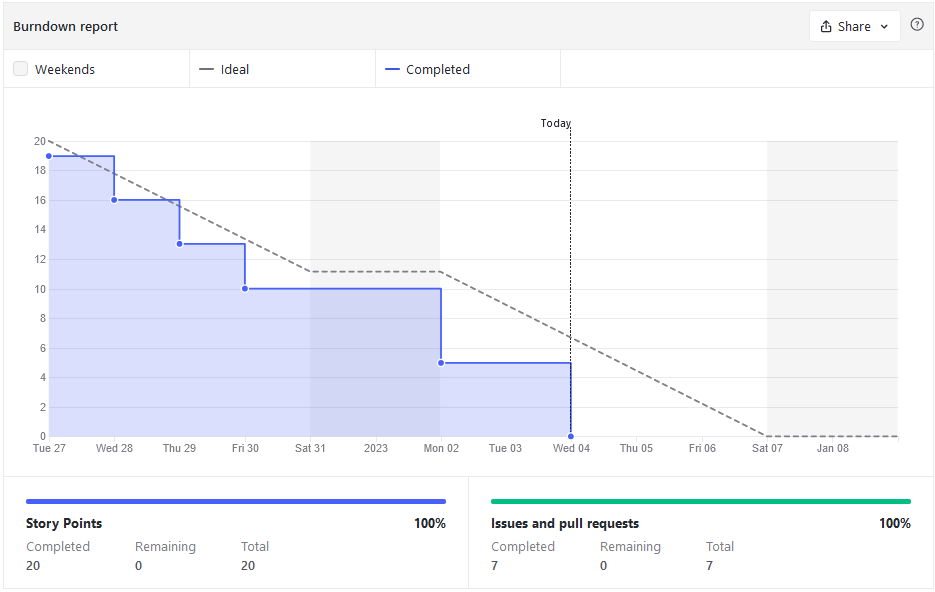
\includegraphics[width=\textwidth]{../img/anexos/bdr/s09_bdr}
	\end{figure}
	
	El número total de horas dedicadas al proyecto fue de $20$. Aunque se <<dejó abierto>> el \textit{sprint} hasta el 8 de enero, la intención era acabarlo el 4 de enero, por lo que la estimación temporal fue correcta.
	
	\item \textbf{\textit{Sprint review meeting}}
	
	Tras haber finalizado la experimentación, se decidió investigar nuevos temas para dedicar el tiempo restante a otros con mejor método de extracción de vectores de características.
	
\end{itemize}

\subsubsection{\textit{Sprint 10: Amchur}}

\begin{itemize}
	\item \textbf{\textit{Planning meeting}}
	
	En este \textit{sprint} se decidió:
	\begin{enumerate}
		\item Lectura de aplicación del semisupervisado a la intrusión de redes: lectura del paper de BigFlow y su mejora semisupervisada. Investigación de la base de datos.
		\item Búsqueda de aplicaciones del semisupervisado a nuevos temas: entre ellos NIDS, \textit{phishing}, detección de \textit{malware}, de \textit{markets} en la \textit{deep web}, de intrusiones en redes IoT, etc. Búsqueda de bases de datos.
		\item Continuación de implementación del \textit{democratic co-learning}: implementación del algoritmo y lectura del paper.
	\end{enumerate}
	\item \textbf{Marcas temporales}		
	
	El \textit{sprint} se desarrolló entre el 9 y el 20 de enero. Fueron dedicadas al \textit{sprint} 9 horas de trabajo. No se incluye un \textit{burndown report} debido a que no se asociaron las horas de investigación a ningún repositorio en concreto.
	
	\item \textbf{\textit{Sprint review meeting}}
	
	Tras haber comentado las distintas ramas de investigación posibles, en esta reunión se decidió cambiar el tema principal a la aplicación del aprendizaje semisupervisado para la detección de \textit{phishing}.
\end{itemize}


\subsubsection{\textit{Sprint 11: Parsley}}
\begin{itemize}
	
	\item \textbf{\textit{Planning meeting}}
	
	Durante esta reunión se acordó comenzar a trabajar en el nuevo objetivo, además de completar documentación pendiente.
	
	\begin{enumerate}
		\item Extracción de vectores de características de URLs:  generar el código que permita diferenciar un enlace de \textit{phishing} de uno verídico.
		\item Pruebas unitarias: debido a que se ha creado una clase de utilidades para apoyar la extracción de los vectores de características, se ha decidido investigar acerca de las pruebas unitarias en Python e implementar algunas.
		\item Creación de instancias de Tor: debido a que algunos de los métodos de los vectores de características requieren hacer peticiones a páginas peligrosas, se ha decidido proteger esas peticiones utilizando instancias de Tor, de manera que se oculte la IP del ordenador que realiza las peticiones. Para ello, se ha creado un \textit{script} capaz de levantar estas conexiones y se han utilizado como \textit{proxies} (protocolo SOCKS5).
		\item Documentación y experimentación: se ha generado la documentación relativa al algoritmo \textit{tri-training}, además de su comparativa y estudio (gráficas).
		\item Refactorización: debido a que muchos de los métodos para realizar las gráficas del \textit{tri-training} duplican código de los utilizados para generar el \textit{co-forest}, se ha decidido realizar métodos comunes y una clase de utilidades para las gráficas.
		
	\end{enumerate}
	\item \textbf{Marcas temporales}	
		
	El \textit{sprint} fue completado entre el 24 y el 30 de enero del 2022.
	
	\item \textbf{\textit{Burndown Report}}
	\begin{figure}[h]
		\caption{\textit{Burndown Report Sprint 11}}
		\centering
		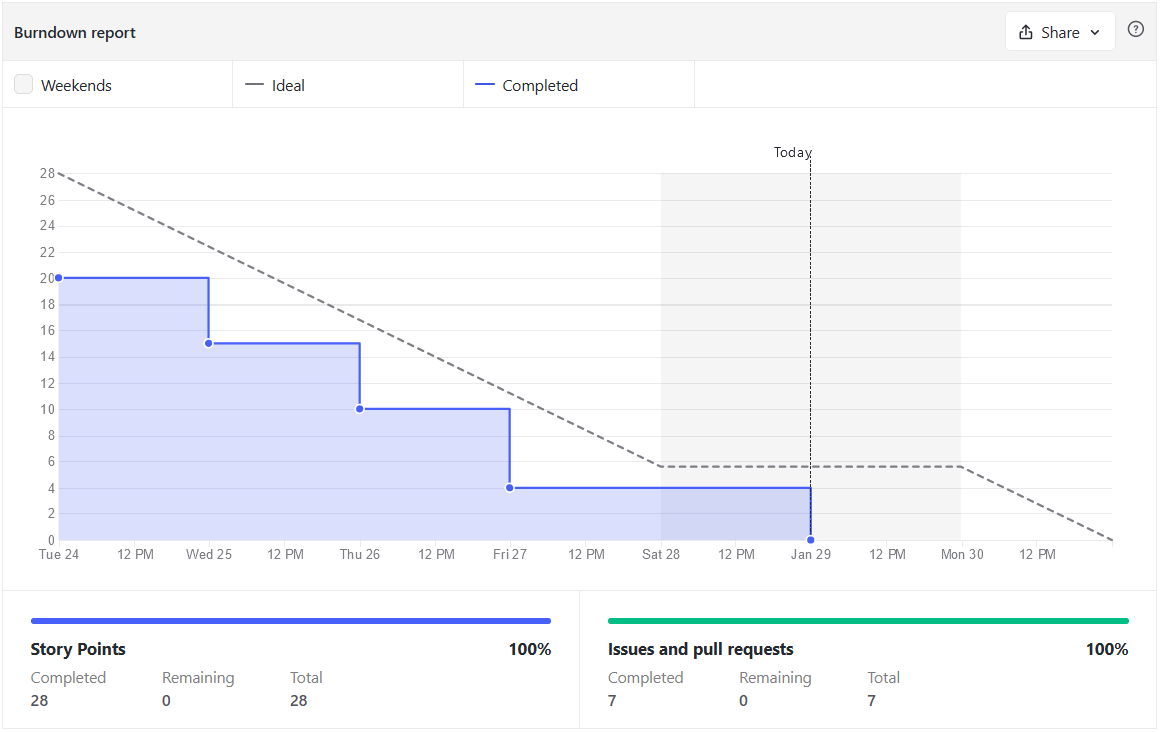
\includegraphics[width=\textwidth]{../img/anexos/bdr/s11_bdr}
	\end{figure}
	
	El número total de horas dedicadas al proyecto fue de $30$, requiriendo una cifra ligeramente inferior a la estimada. Aún así se cerró antes de tiempo debido a que se pudieron invertir más horas por día de las predichas. Nuevamente, recalcar que el tiempo sobrante en ciertos \textit{issues} fue destinado a la generación de vectores de características.
	
	\item \textbf{\textit{Sprint review meeting}}
	
	En la reunión se concluyó que el trabajo desarrollado es correcto, a excepción de un detalle a cambiar respecto al algoritmo TF-IDF.
	
\end{itemize}
\subsubsection{\textit{Sprint 12: Oregano}}
\begin{itemize}
	
	\item \textbf{\textit{Planning meeting}}
	
	En este \textit{sprint} se decidió, principalmente, avanzar la documentación. Por lo tanto, se acordó:
	\begin{enumerate}
		\item Documentar los resultados de la aplicación de \textit{machine learning} a la detección de ataques en sistemas de recomendación.
		\item Documentar la parte teórica de ciberseguridad, protocolos (SOCKS5), Tor, etc., además de la creación del \textit{script} para levantar instancias.
		\item Documentar y realizar la comparativa del \textit{tri-training}.
		\item Documentar algunas de las herramientas utilizadas hasta ahora.
		\item Documentar la generación de vectores de características para la detección de phishing, además de revisar el código.
	\end{enumerate}
	
	Adicionalmente se solucionaron algunos aspectos no relacionados con la documentación:
	
	\begin{enumerate}
		\item Arreglar el uso del algoritmo TF-IDF e integrarlo en la generación de vectores para la detección de \textit{phishing}.
		\item Creación de métodos que recopilen las URLs de las que se extraerán los vectores de características, además de depurar algunos de los \texttt{csv} que se necesitan para los enlaces persistentes.
	\end{enumerate}
	
	\item \textbf{Marcas temporales}		
	
	El \textit{sprint} se desarrolló entre el 31 de enero y el 6 de febrero del 2023.
	
	\item \textbf{\textit{Burndown Report}}
		\begin{figure}[h]
		\caption{\textit{Burndown Report Sprint 12}}
			\centering
			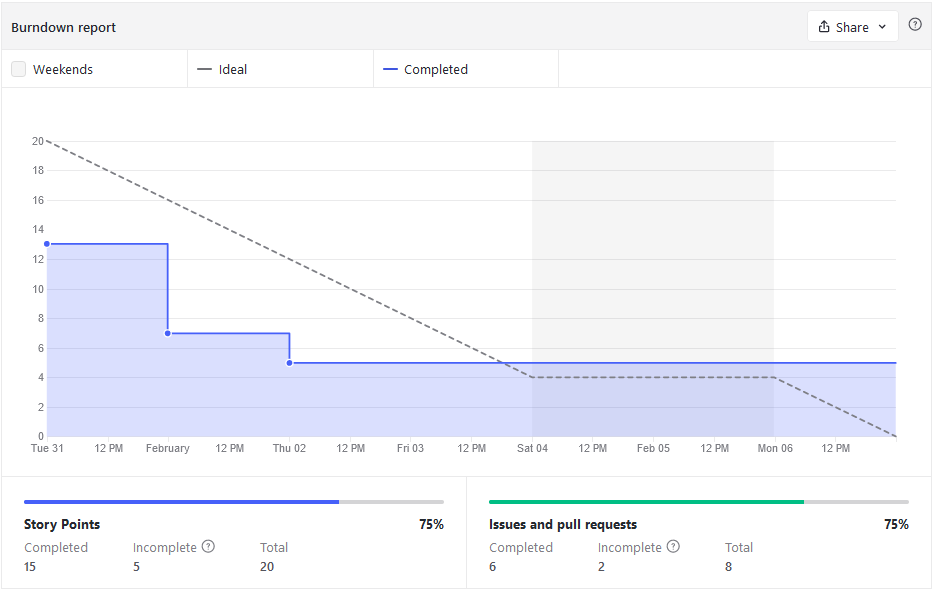
\includegraphics[width=\textwidth]{../img/anexos/bdr/s12_bdr}
		\end{figure}
		
		En este \textit{sprint}, no se pudieron cerrar todos los \textit{issues} planeados debido a que algunos de los completados requirieron más tiempo de lo estimado (por ejemplo, los métodos de obtención de URLs debido a que un servidor bloqueó la IP del equipo por exceso de peticiones o la comparativa del \textit{tri-training} debido a que se decidió cambiar la estética de las gráficas de toda la memoria).
		
	\item \textbf{\textit{Sprint review meeting}}
	
	Tras haber resuelto los problemas que surgieron en el \textit{sprint} y revisado la documentación, se decidió continuar con el proyecto.
	\end{itemize}




\subsubsection{\textit{Sprint 13: Tandoori Masala}}

\begin{itemize}
	\item \textbf{\textit{Planning meeting}}
	
	En este \textit{sprint} se decidió continuar con el algoritmo \textit{democratic-co} learning, además de seguir documentando e iniciar el control de calidad.
	
	\begin{enumerate}
		\item Implementar el \textit{democratic-co learning} y documentarlo en la sección teórica.
		\item Documentar la extracción de vectores de características de \textit{phishing}, ataques \textit{web} típicos, la sección teórica del \textit{phishing}, los anexos e incluir las correcciones realizadas por el tutor.
		\item Renombrar el repositorio y adaptar la memoria a la nueva sección de \textit{phishing}: modificar introducción, trabajos relacionados etc.
		\item Crear ilustraciones para mejorar la memoria, además de modificar las existentes con el fin de incluirlas en formato \texttt{pdf} para mejorar la calidad.
		\item Revisar la extracción de vectores de características para \textit{phishing} (\textit{features} 1-7).
		\item Vincular el repositorio con Sonarcloud e implementar control de calidad. Cambiar el archivo \texttt{README.md} e incluir nuevos \textit{badges}.
	\end{enumerate}
	\item \textbf{Marcas temporales}		
	
	El \textit{sprint} fue desarrollado entre el 7 y el 13 de febrero de 2022.
	
	\item \textbf{\textit{Burndown Report}}
	
	\begin{figure}[h]
		\caption{\textit{Burndown Report Sprint 13}}
		\centering
		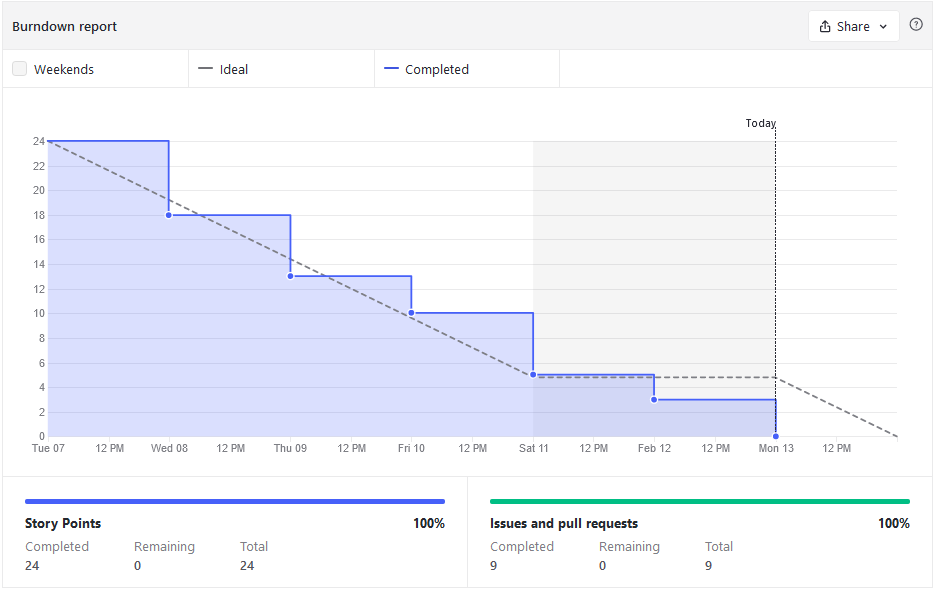
\includegraphics[width=\textwidth]{../img/anexos/bdr/s13_bdr}
	\end{figure}

	En este \textit{sprint} todos los \textit{issues} fueron cerrados. Al igual que en ocasiones anteriores, aunque la estimación particular de cada tarea pudo no ser correcta, en general la de todo el \textit{sprint} resultó equilibrada. Se calcula que el tiempo real dedicado al proyecto fue ligeramente superior, de unas 26 horas. Esto es debido principalmente a que se dedicó tiempo a la revisión <<estilística>> de la memoria (corrección de cursivas incorrectas, nombres propios, anglicismos, etc.).

	\item \textbf{\textit{Sprint review meeting}}
	
	Lo más destacable es la corrección de ciertos aspectos relacionados con el \textit{democratic-co learning}. Por ello, se estimó que debían ser corregidos.
\end{itemize}


\subsubsection{\textit{Sprint 14: Chimichurri}}
\begin{itemize}
	\item \textbf{\textit{Planning meeting}}
	
	Se decidió trabajar en:
	\begin{enumerate}
		\item Corrección de los vectores de características de \textit{phishing} y de la API de extracción de enlaces. Generación de \textit{dataset} parcial y gráficas de pruebas para comprobar el nivel de detección de la propuesta.
		\item Documentar algún aspecto pendiente. En especial herramientas nuevas, anexos y el proceso de minería de datos (realizar ilustraciones).
		\item Introducir DeepSourceBot y mejorar la calidad del proyecto (corregir defectos de código). Proteger las ramas del repositorio para prevenir posibles conflictos con el \textit{bot}.
		\item Incluir Travis CI y generar una \textit{build} de \textit{tests}. Reorganizar el proyecto en estructura de paquetes.
		\item Corregir el \textit{democratic-co learning}, realizar la comparativa contra sslearn y documentar los resultados. 
		\item Lanzar los primeros experimentos de detección de \textit{phishing} y corregir posibles \textit{bugs}.
	\end{enumerate}

	\item \textbf{Marcas temporales}		
	
	El \textit{sprint} fue desarrollado entre el 14 y el 20 de febrero de 2022.
	
	
	\item \textbf{\textit{Burndown Report}}
	
		\begin{figure}[h]
		\caption{\textit{Burndown Report Sprint 14}}
		\centering
		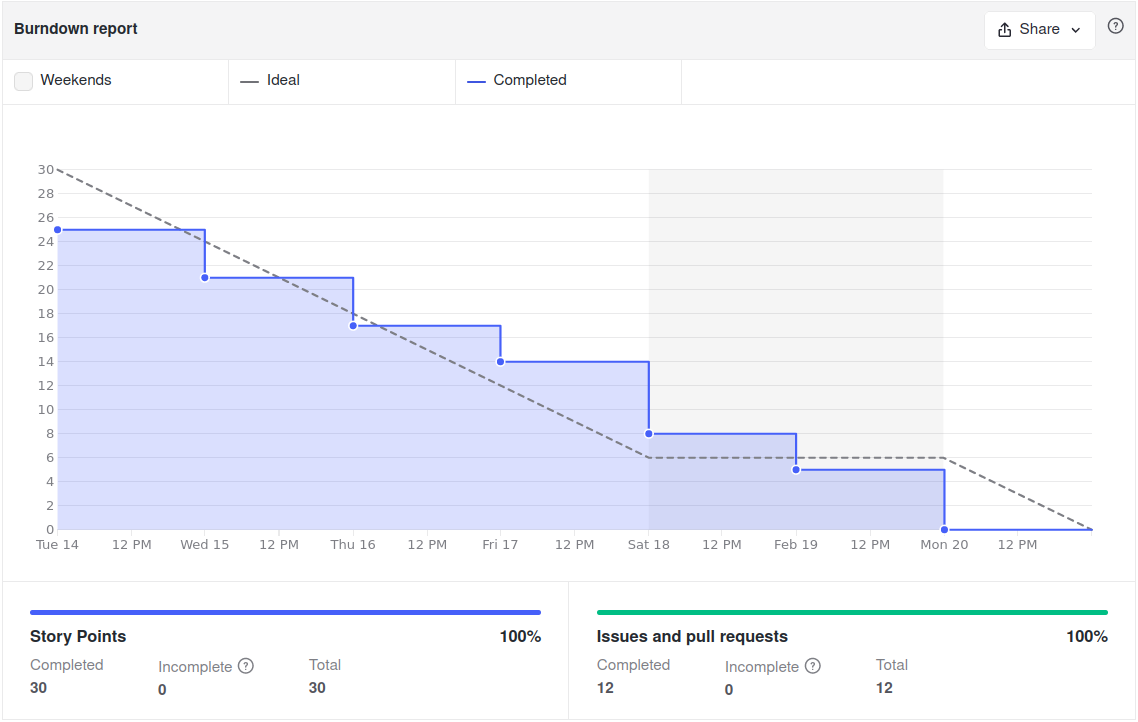
\includegraphics[width=\textwidth]{../img/anexos/bdr/s14_bdr}
	\end{figure}

	En este \textit{sprint} se concluyó el trabajo propuesto. Debido a que hubo ciertas dificultades, se calcula que la estimación real del trabajo es de 33 horas.


	\item \textbf{\textit{Sprint review meeting}}
	
	En el \textit{feedback} se estimó que los algoritmos de semisupervisado están correctamente implementados y se decidió avanzar otros aspectos del proyecto.
\end{itemize}


\subsubsection{\textit{Sprint 15: Anise}}
\begin{itemize}
	\item \textbf{\textit{Planning meeting}}
	
	Se decidió trabajar en:
	\begin{enumerate}
		\item Comienzo de la \textit{web}: aprender a utilizar Flask y desarrollar la aplicación. Manejar archivos \texttt{.css} básicos y aprender a usar (por encima) ciertas librerías como Bootstrap, SQL Alchemy, Flask WTF, etc. Búsqueda de una plantilla atractiva y desplegable.
		\item Sistema de bases de datos: buscar servidor (comparativa entre MariaDB y PostgreSQL) y desplegar en local.
		\item Despliegue: despliegue en Heroku y gestión de errores. Levantar tanto la \textit{web} como la base de datos.
		\item Documentación: corrección de aspectos indicados por el tutor, redacción de anexos, inclusión del apartado <<técnicas>> en la memoria principal.
		\item Experimentación: generación del \textit{dataset} real de \textit{phishing} (2\,000 instancias) y realización de las gráficas con datos reales. Posible búsqueda de alternativas a la generación de vectores.
		\item Calidad: corrección de \textit{issues} utilizando Deep Source Bot.
		\item Diagramas: comenzar a realizar diagramas de casos de uso, clases, etc.
		
	\end{enumerate}
	\item \textbf{Marcas temporales}		
	
	El \textit{sprint} fue desarrollado entre el 23 de febrero y el 6 de marzo de 2022.
	
	\item \textbf{\textit{Burndown Report}}
	
	\begin{figure}[h]
		\caption{\textit{Burndown Report Sprint 15}}
		\centering
		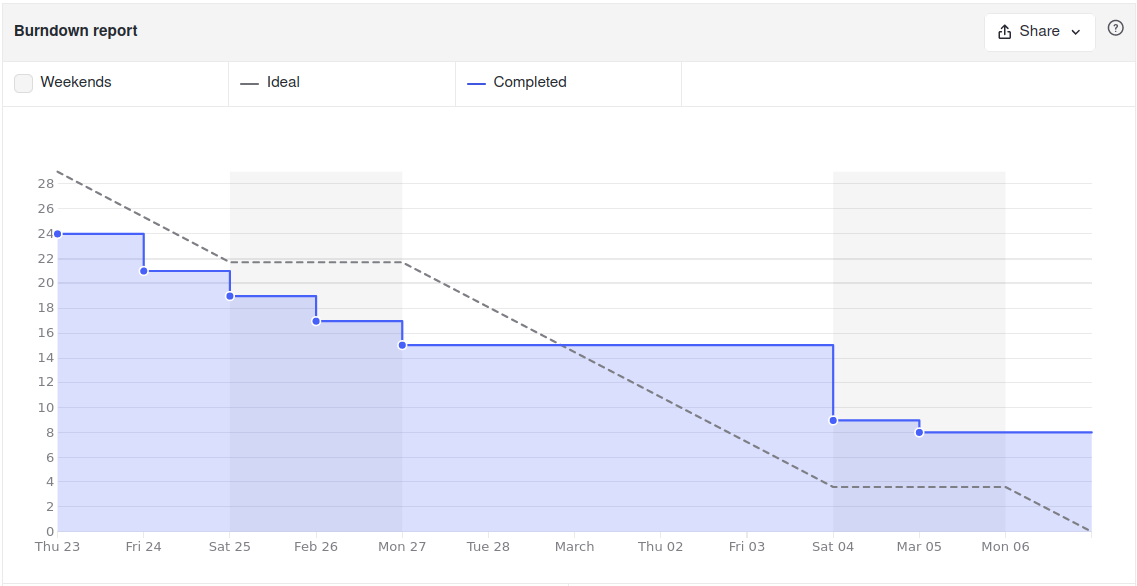
\includegraphics[width=\textwidth]{../img/anexos/bdr/s15_bdr}
	\end{figure}
	
	El tiempo estimado de trabajo fue de 29 horas. Sin embargo, el tiempo real ha sido de 37.5 horas, y no todos los \textit{issues} pudieron ser cerrados. En concreto, se decidió posponer la búsqueda de nuevas formas de generar vectores de características por los buenos resultados reportados y no se dedicó tanto tiempo como el esperado a la generación de diagramas (únicamente se realizó el de casos de uso).
	
	Claramente se subestimó el tiempo requerido en realizar pantallas \textit{web}, desplegar en Heroku y gestionar servidores de bases de datos. Hubo complicaciones debido a que se ha escogido una plantilla profesional, y el uso del lenguaje es complejo. Todavía hay ciertos aspectos que arreglar respecto al despliegue en Heroku (no renderiza correctamente los menús desplegables a diferencia de <<local>>).
	
	\item \textbf{\textit{Sprint review meeting}}
	
	En esta reunión se concluyó que el incremento había sido desarrollado correctamente con la excepción de los diagramas (debido a que se dedicó poco tiempo). Por lo tanto, se ofreció retroalimentación con respecto a los mismos con el fin de volverlos a generar. También se recibió \textit{feedback} relacionado con la documentación.
\end{itemize}


\subsubsection{\textit{Sprint 16: Vanilla}}
\begin{itemize}
	
	\item \textbf{\textit{Planning meeting}}
	
	En esta reunión se plantearon los siguientes objetivos:
	\begin{enumerate}
		\item Diagramas: repetir el diagrama de casos de uso partiendo de la retroalimentación proporcionada por el \textit{product owner}. Realizar el diagrama de clases de la base de datos relacional y generar \textit{mockups} de las interfaces para la página \textit{web}.
		\item \textit{Web}: implementación de funcionalidad. Serialización y deserialización de clasificadores, generación de funciones de utilidades para modularizar el ML y diseño de la interacción entre elementos (comunicación en variables de sesión, formularios nuevos, etc.). Nuevas pantallas (carga con animaciones para tareas que requieran más tiempo), adaptación del modelo de datos de la \textit{web} al nuevo diagrama de clases e introducción de roles y permisos. Pantallas asociadas al administrador (esqueleto realizado y adaptación del menú). Mejoras estilísticas (segmentos utilizados, usuarios activos, \textit{badges} y más) y corrección de errores (encabezados y sesiones activas). Implementación definitiva de los modelos de la base de datos (sustituidos los anteriores por no ser suficiente para cubrir los nuevos requerimientos).
		\item Documentación: corregir aspectos previos y realizar anexos. Introducir las secciones de CD/CI, Gitflow, Scrum y complementar las herramientas. Planificación temporal del \textit{sprint}.
		\item Herramientas: realizar una primera <<toma de contacto>> con \texttt{D3.js} y decidir si merece la pena introducir esta tecnología en la página \textit{web}.
		
	\end{enumerate}
	\item \textbf{Marcas temporales}
	
	El \textit{sprint} fue desarrollado entre el 7 de marzo y el 13 de marzo del 2023.
			
	\item \textbf{\textit{Burndown Report}}
	
	\begin{figure}[h]
		\caption{\textit{Burndown Report Sprint 16}}
		\centering
		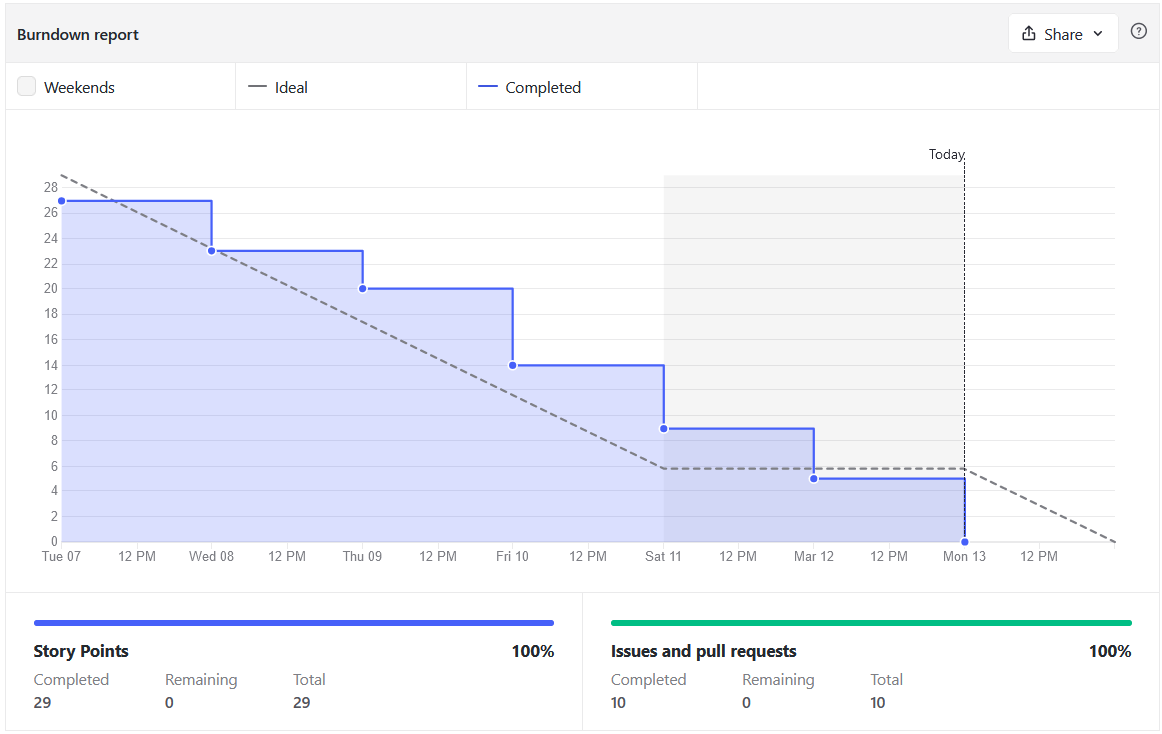
\includegraphics[width=\textwidth]{../img/anexos/bdr/s16_bdr}
	\end{figure}

	En este \textit{sprint} todos los \textit{issues} fueron cerrados. Se estimó un tiempo total de trabajo de 29 horas y el tiempo real dedicado ha sido de 30 horas. Cabe destacar que los \textit{issues} de realización de \textit{mockups} requirieron menos tiempo del estimado y que el tiempo sobrante se empleó en seguir programando la página \textit{web}.
	
	Aunque no estaba planificado, también se incluyó la tecnología GitGuardian en el flujo de Git con el fin de proteger la aplicación ante posibles filtraciones de contraseñas (en concreto, de la base de datos).

	\item \textbf{\textit{Sprint review meeting}}
	
	En esta reunión se concluyó que todos los \textit{issues} fueron desarrollados correctamente a excepción de los diagramas (puesto que se realizó directamente un diagrama de <<clases>> para una base de datos en lugar de realizar la progresión correcta, es decir, entidad-relación, relacional, etc.). Por ello, se estimó conveniente repetir los diagramas.
\end{itemize}


\subsubsection{\textit{Sprint 17: Sriracha}}
\begin{itemize}
	
	\item \textbf{\textit{Planning meeting}}
	
	En esta reunión se decidió realizar un \textit{sprint} más largo para avanzar en la funcionalidad general de la \textit{web}. Para ello, se plantearon los siguientes objetivos:
	\begin{enumerate}
		\item Diagramas: corregir pequeños aspectos del diagrama de casos de uso, realizar el diagrama entidad-relación y el relacional de la base de datos. Redactar el diccionario de datos.
		\item \textit{Web}: implementación de funcionalidad vinculada con el nuevo modelo de datos (cambiar la base de datos anterior). Completar un \textit{dashboard} funcional (con gráficas y que realice la extracción del vector de características, además de mostrar cómo se ha logrado y estadísticas de las URLs analizadas). Iniciar la administración de modelos e implementar la interfaz principal y el formulario de creación de nuevos modelos desde la web (con funcionalidad, serializando los modelos generados en cada petición). Programar la interfaz principal de administración de instancias (consultas paginadas con formularios de \textit{checkboxes}) y generar \texttt{csv} compatibles (y descargables) con el entrenamiento de modelos.
		\item Herramientas: generar archivos de utilidades (refactorizar) y permitir la subida de archivos al servidor y la descarga desde el mismo. Corregir el \textit{select all} del menú principal y hacerlo estético. Hacer comprobación de \textit{emails} propia y eliminar la dependencia, además de asegurar que los formularios no dejen avanzar si no están completados los datos requeridos.
		\item Documentación: corregir aspectos previos y realizar anexos. Documentar el despliegue en Heroku, revisar la memoria (en busca de posibles pérdidas de información), corregir el \textit{mockup} del \textit{dashboard} y repasar los trabajos relacionados.
		\item Semisupervisado: revisar el \textit{feedback} proporcionado por Álvar Arnaiz y César Ignacio García acerca de la inicialización del parámetro $w$ en el \textit{co-forest}. Corregir el código, repetir experimentos y documentar los resultados.
		\item Calidad: corregir defectos de código.
		\item Despliegue: desplegar el repositorio desde raíz (en lugar de sólo la \textit{web}) y cambiar las dependencias (minimizando al máximo y solucionando incompatibilidades) del \texttt{requirements.txt}.
		
	\end{enumerate}
	\item \textbf{Marcas temporales}
	
	El \textit{sprint} fue desarrollado entre el 14 de marzo y el 28 de marzo del 2023.
	
	\item \textbf{\textit{Burndown Report}}
	
	\begin{figure}[h]
		\caption{\textit{Burndown Report Sprint 17}}
		\centering
		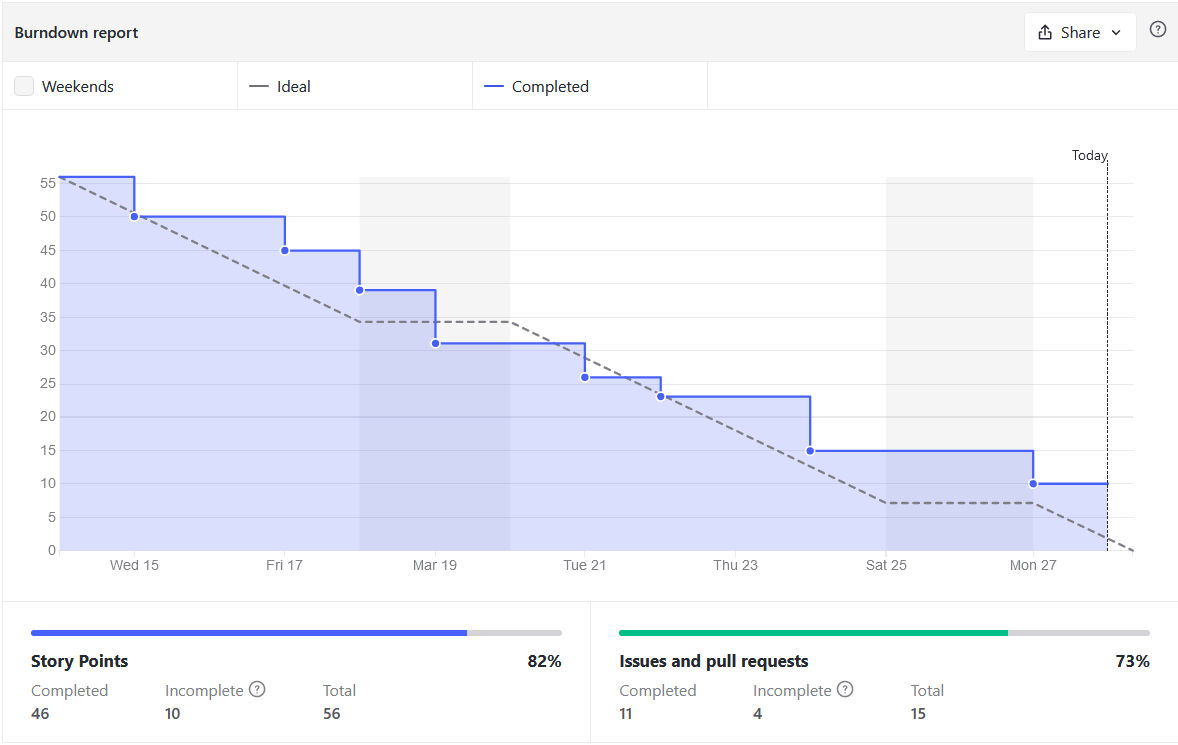
\includegraphics[width=\textwidth]{../img/anexos/bdr/s17_bdr}
	\end{figure}
	
	En este \textit{sprint} no se consiguió cerrar todos los \textit{issues} planificados.
	
	Los diagramas y la redacción del diccionario de datos requirieron el doble de tiempo del estimado debido a las múltiples revisiones (con sus respectivas correcciones) por parte del tutor y otros profesores (Jesús Maudes).  Además, se subestimó completamente el tiempo requerido en la realización de la \textit{web} y, aunque se cerraron los \textit{issues}, algunos de ellos se implementaron de forma <<optimista>> (falta <<hacer segura>> la implementación mediante comprobaciones de tipos, tratamiento de excepciones, etc.).
	
	Por este motivo, no se cerraron los ítems 5, 6 y 7 y únicamente se documentaron los anexos (dentro del ítem 4). El tiempo real dedicado a la realización del \textit{sprint} ha sido de 52.5 horas.
	
	\item \textbf{\textit{Sprint review meeting}}
	
	En esta reunión se revisó la nueva funcionalidad implementada. El \textit{product owner} sugirió algunas mejoras dentro de cada pantalla mostrada. Las más destacables: internacionalizar la \textit{web}, añadir nuevas funcionalidades (gráficos en el \textit{dashboard}, pseudocódigos en la creación de modelos, etc.). Además, se revisaron los diagramas realizados hasta el momento dándolos por válidos y se propuso empezar a documentar los nuevos.
	
\end{itemize}



\subsubsection{\textit{Sprint 18: Nutmeg}}
\begin{itemize}
	\item \textbf{\textit{Planning meeting}}
	
	Hasta este \textit{sprint} se ha conseguido implementar una \textit{web} con funcionalidad mínima. Se ha decidido que, durante los 4 siguientes, se dedicará un \textit{sprint} a cada sección de la \textit{web} para implementar la funcionalidad al completo y realizar la documentación disponible en estos anexos. Por lo tanto, \textit{sprint} 18 se ha dedicado al \textit{index}, a la página de reportar URLs y al \textit{dashboard}. Aprovechando las vacaciones se ha decidido, además, integrar toda la documentación atrasada e introducir nuevos experimentos para el \textit{co-forest}.
	
	\begin{enumerate}
		\item \textit{Web}: finalizar el \textit{index} (mostrar solo modelos visibles, controlar las excepciones, corección de URLs por parte del usuario, introducir el análisis rápido, modificar la interfaz), mejorar el \textit{dashboard} (espaciado en las fórmulas, introducir botón de notificar análisis incorrectos, añadir un gráfico interactivo global con las métricas para todos los clasificadores, arreglar ejes de los gráficos y añadir las métricas F1 y ROC AUC) y arreglar la página para reportar URLs (adaptar al modelo de datos tras las nuevas correcciones).
		\item Calidad y experiencia de usuario (UX): mejorar la documentación del código, arreglar \textit{code smells} e incluir pantallas llamativas de carga y error (con ilustraciones del robot adaptadas a cada situación).
		\item Anexos: documentar los casos de uso correspondientes a este \textit{sprint}, corregir el diccionario de datos (nueva columna y tamaños), incluir en la memoria los diagramas hasta ahora realizados (E-R, relacional, CU) y comentarlos. Redactar anexo~\ref{s:anexo-B} (requisitos funcionales). Realizar los digramas de secuencia del \textit{index} y de la página de reportar URLs y redactar explicación. Realizar diagrama de clases.
		\item Documentación: incluir algoritmos de \textit{hash} y revisar la memoria en busca de la información <<desaparecida>> (encontrado error en el \textit{commit} \href{https://github.com/phf1001/semisupervised-learning-in-cibersecurity/commit/66d22ac0cf9ffc24385656ae85bf831e03f924be}{\texttt{66d22ac}}).
		\item{Experimentación}: evaluar como la inicialización del vector \texttt{previous\_w} afecta al rendimiento del algoritmo \textit{co-forest}.
		
	\end{enumerate}
	\item \textbf{Marcas temporales}		
	
	El \textit{sprint} se ha desarrollado entre el 29 de marzo y el 8 de abril del 2023.
	
	\item \textbf{\textit{Burndown Report}}
	
		\begin{figure}[h]
		\caption{\textit{Burndown Report Sprint 18}}
		\centering
		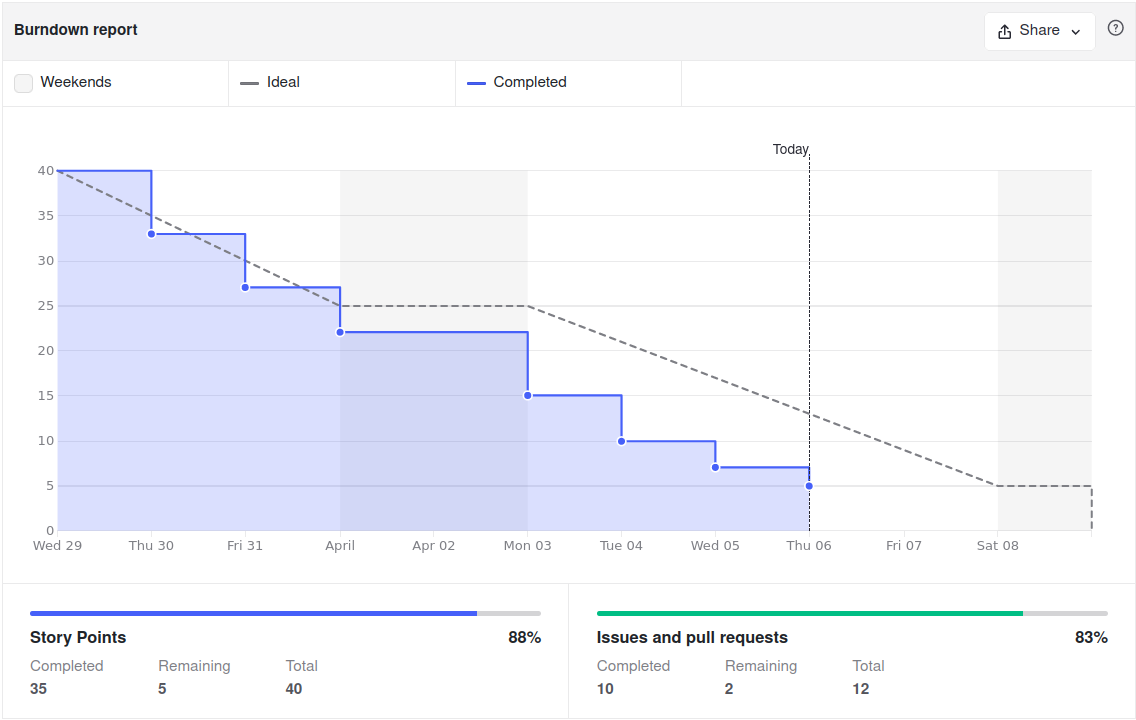
\includegraphics[width=\textwidth]{../img/anexos/bdr/s18_bdr}
	\end{figure}

	Como se puede comprobar, durante este \textit{sprint} se han conseguido cerrar todos los \textit{issues} propuestos. Si bien es cierto que el tiempo de programación estimado fue superior al real, se dedicó el tiempo sobrante a la mejora de calidad de código.
	
	Por otro lado, aprovechando las vacaciones, se decidió invertir más tiempo del planeado para avanzar el proyecto (redactando la mayoría del anexo~\ref{s:anexo-B} aunque en un principio no estuviese planificado). Por lo tanto, de las 40 horas que se estimaron, se realizó un trabajo real de 47 horas.


	\item \textbf{\textit{Sprint review meeting}}
	
	Como se ha ido documentando en los \textit{issues} de GitHub\footnote{\url{https://github.com/phf1001/semisupervised-learning-in-cibersecurity/issues/115}}, lo más relevante ha sido la experimentación con el \textit{co-forest}, ya que se piensa que la inicialización del vector \texttt{previous\_w} tiene un impacto real mayor que el estimado en el desempeño del algoritmo. Por ello, se ha planificado una experimentación a gran escala para cuando la \textit{web} se finalice. Respecto a la \textit{web}, se han comentado ciertas sugerencias de mejora (colores en las etiquetas, etc.).
	
\end{itemize}


\subsubsection{\textit{Sprint 19: Panch Phoran}}
\begin{itemize}
	\item \textbf{\textit{Planning meeting}}
	
	El \textit{sprint} 19 se ha dedicado a las instancias, a la administración de modelos y a la revisión de sugerencias y notificaciones, además de mejorar la calidad del código y arreglar defectos existentes.
	
	\begin{enumerate}
		\item \textit{Web}: finalizar toda la funcionalidad relacionada con modelos, instancias y administración de \textit{reports}. Corregir defectos de código, refactorizar y modificación de constantes (archivo de configuración).
		\item Calidad y UX: mejorar la documentación del código e iniciar la internacionalización (instalación y configuración de Babel).
		\item Anexos: documentar los casos de uso correspondientes a este \textit{sprint}, corregir el diagrama de casos de uso (y los requisitos) con las nuevas funcionalidades, incluir el \textit{feedback} proporcionado por el tutor en los anexos y actualizar el diagrama relacional junto con el diccionario de datos (incluir \texttt{CASCADES} y otras correcciones menores).
		
	\end{enumerate}
	\item \textbf{Marcas temporales}		
	
	El \textit{sprint} se ha desarrollado entre el 10 y el 23 de abril del 2023.
	
	\item \textbf{\textit{Burndown Report}}
	
	\begin{figure}[h]
		\caption{\textit{Burndown Report Sprint 19}}
		\centering
		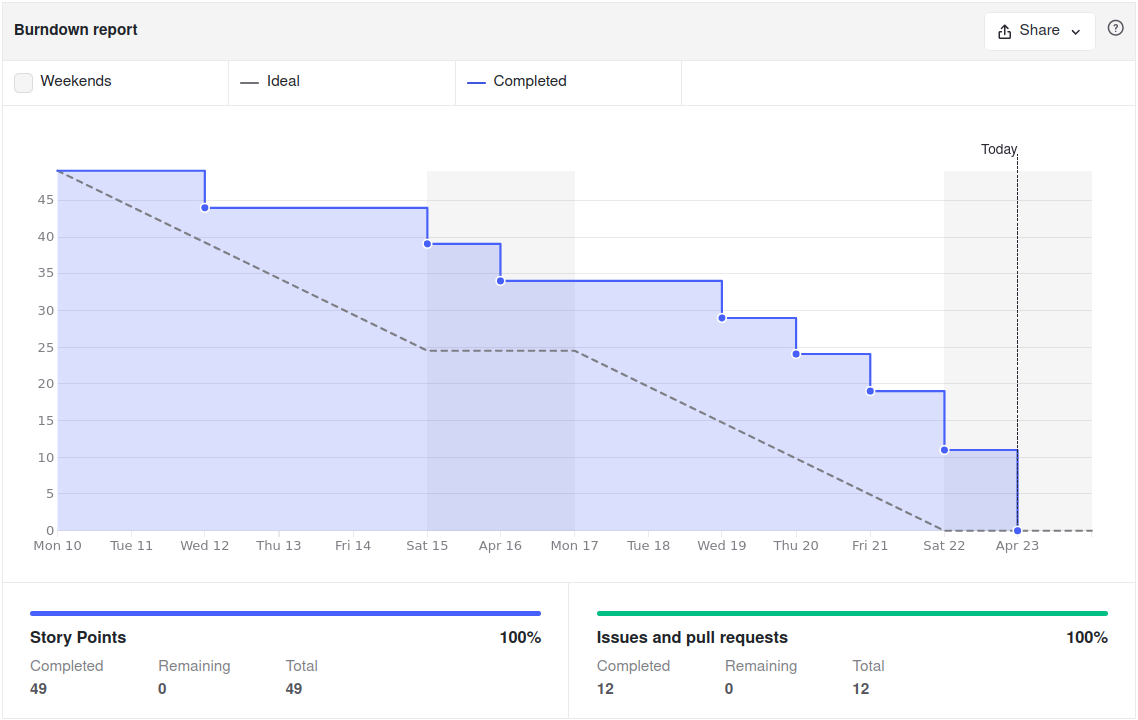
\includegraphics[width=\textwidth]{../img/anexos/bdr/s19_bdr}
	\end{figure}
	
	Como se puede comprobar, durante este \textit{sprint} se ha conseguido cerrar todos los \textit{issues} propuestos, habiendo dedicado un mayor tiempo al proyecto durante la segunda semana. El tiempo estimado ha sido de 49 horas, habiéndose dedicado un real de 48 horas y media.
	
	\item \textbf{\textit{Sprint review meeting}}
	
	...
	
\end{itemize}




\subsubsection{\textit{Sprint N: }}
\begin{itemize}
	\item \textbf{\textit{Planning meeting}}
	\begin{enumerate}
		\item
		\item
		\item
		\item 
	\end{enumerate}
	\item \textbf{Marcas temporales}		
	\item \textbf{\textit{Burndown Report}}
	\item \textbf{\textit{Sprint review meeting}}
\end{itemize}



\section{Estudio de viabilidad}

\subsection{Viabilidad económica}

\subsection{Viabilidad legal}


